\documentclass[10pt,noamssymb,svgnames]{beamer}
\usetheme{metropolis}

\usepackage{bm}
\usepackage{amsmath}
\usepackage{amssymb}
\usepackage{booktabs}
\usepackage{ragged2e}
\usepackage[vlined]{algorithm2e}
\usepackage[absolute,overlay]{textpos}
\usepackage{tikz}
\usetikzlibrary{shapes.geometric,arrows}

\tikzset{onslide/.code args={<#1>#2}{%
  \only<#1>{\pgfkeysalso{#2}} % \pgfkeysalso doesn't change the path
}}
\tikzset{temporal/.code args={<#1>#2#3#4}{%
  \temporal<#1>{\pgfkeysalso{#2}}{\pgfkeysalso{#3}}{\pgfkeysalso{#4}} % \pgfkeysalso doesn't change the path
}}

\usepackage{hyperref}
\hypersetup{colorlinks=true,urlcolor=cyan,linkcolor=}

\definecolor{CyanBlueAzure}{HTML}{4B8BBE} % light blue
\definecolor{LapisLazuli}{HTML}{306998} % dark blue

% BEAMER CONFIGURATION ---------------------------------------------------------
\newcommand<>{\blue}[1]{{\color#2{blue}#1}}
\setbeamerfont{block title}{size=\normalsize}
\setbeamerfont{block body}{size=\scriptsize}
\setbeamertemplate{mini frames}{}

%\setbeamercolor{sectiontitle}{fg=black}
\setbeamercolor{part title}{fg=black}
\setbeamercolor{progress bar}{fg=CyanBlueAzure}
\setbeamercolor{progress bar in head/foot}{fg=LapisLazuli,bg=CyanBlueAzure}
\setbeamercolor{progress bar in section page}{fg=LapisLazuli,bg=CyanBlueAzure}
\setbeamercolor{frametitle}{bg=black!75!white}

% Configure progress bars
\metroset{progressbar=frametitle}
\makeatletter
\setlength{\metropolis@progressonsectionpage@linewidth}{1pt}
\setlength{\metropolis@progressinheadfoot@linewidth}{2pt}
\makeatother

% Blank footnote
\newcommand\blfootnote[1]{%
  \begingroup
  \renewcommand\thefootnote{}\footnote{#1}%
  \addtocounter{footnote}{-1}%
  \endgroup
}

\bibliographystyle{ans}
\setbeamertemplate{bibliography item}{\insertbiblabel}

\newcommand{\highlight}[1]{%
  \colorbox{yellow!20}{$\displaystyle#1$}}

% TIKZ CONFIGURATION -----------------------------------------------------------
\tikzstyle{start} = [rectangle, draw, fill=green!20, rounded corners=3mm,
  centered, minimum height=1em]
\tikzstyle{end} = [rectangle, draw, fill=red!20, rounded corners=3mm,
  centered, minimum height=1em]
\tikzstyle{process} = [rectangle, draw, fill=yellow!20, text width=8em, text
  centered, minimum height=1em]
\tikzstyle{decision} = [diamond, draw, fill=gray!20, text width=5em, text badly centered,
  inner sep=0pt]
\tikzstyle{line} = [draw, -latex', thick]

%%---------------------------------------------------------------------------%%
\title{OpenMC Course Introduction}
\author{Joint ICTP-IAEA Workshop on Open-Source Nuclear Codes for Reactor Analysis \\ August 7-11, 2023}
%\institute{Argonne National Laboratory}
\date{}
\titlegraphic{
  \begin{picture}(0,0)
    \put(325,-220){\makebox(0,0)[rt]{
\includegraphics[height=0.75cm]{../images/openmc_logo.png}}}
    \put(20,-215){\makebox(0,0)[rt]{
\includegraphics[height=0.9cm]{../images/International_Centre_for_Theoretical_Physics.png}}}
    \put(60,-215){\makebox(0,0)[rt]{
\includegraphics[height=0.9cm]{../images/International_Atomic_Energy_Agency_Logo.png}}}
  \end{picture}}

%%---------------------------------------------------------------------------%%
\begin{document}

\maketitle

%%---------------------------------------------------------------------------%%
\section{Course Logistics}

\begin{frame}{Logistics}
  Instructors: Jiwon Choe (KAERI) \& Patrick Shriwise (ANL)
  \vfill Asking Questions:
  \begin{itemize}
    \item In-person
    \item Chat on Zoom (during sessions)
  \end{itemize}
\end{frame}

\begin{frame}{Interactive Sessions}
  \begin{itemize}
    \item You will be using \textbf{Jupyter Lab} for demonstrations and
    (optionally) take-home exercises
    \item Instructor will give live demo for each session, and you can follow
    along in your own Jupyter Lab instance (dual monitor / side-by-side)
    \item The URL provided to you will be available all week but will be
    shutdown at the end of the week --- ``notebooks'' can be downloaded at
    anytime
  \end{itemize}
\end{frame}

%%---------------------------------------------------------------------------%%
\section{Monte Carlo Basics}

\begin{frame}{Monte Carlo Particle Transport}
  \begin{itemize}
  \item Analysis of nuclear reactors, fusion devices, radiation shielding, and
    other problems relies on ability to solve particle transport equations
    \begin{itemize}
    \item \emph{Deterministic methods:} discrete ordinates, method of
      characteristics, collision probability method, diffusion theory
    \item \emph{Monte Carlo (MC) method:} directly simulate life of individual
      particles using known probability distributions
    \end{itemize}
  \item MC method confers a number of benefits:
    \begin{itemize}
    \item Use of continuous-energy interaction data (no grouping necessary)
    \item No spatial approximations necessary
    \item Parallelization is ``simple'' since particles do not interact with one
      another
    \item Some classes of problems are very difficult to solve at all with
    deterministic methods (e.g., high-energy physics)
    \end{itemize}
  \item Biggest impediment to wider use is \emph{time to solution}
  \end{itemize}
\end{frame}

\begin{frame}{Neutral particle transport}
  \centering
  \resizebox{\textwidth}{!}{%
  \begin{tikzpicture}[node distance=2cm]
    \node[start] (source) {Sample source $\bm{r}, \bm{\Omega}, E$};
    \node[process, below of=source, node distance=1.8cm] (db) {Sample distance to boundary, $d_b$};
    \node[process, below of=db] (dc) {Sample distance to collision, $d_c$};
    \node[decision, below of=dc, node distance=2.3cm] (dbdc) {$d_b < d_c$?};

    \node[process, right of=dbdc, node distance=4cm] (boundary) {Cross boundary};
    \node[decision, above of=boundary, node distance=2.3cm] (leak) {Leak?};
    \node[end, right of=leak, node distance=3cm] (leaked) {End};

    \node[process, left of=dbdc, node distance=4cm] (collision) {Sample nuclide / reaction};
    \node[decision, above of=collision, node distance=2.3cm] (absorb) {Absorption?};
    \node[end, left of=absorb, node distance=3cm] (dead) {End};
    \node[process, above of=absorb] (secondary) {Sample $\bm{\Omega'}, E'$};

    \path[line] (source) -- (db);
    \path[line] (db) -- (dc);
    \path[line] (dc) -- (dbdc);
    \path[line] (dbdc) -- node[above] {yes} (boundary);
    \path[line] (dbdc) -- node[above] {no} (collision);
    \path[line] (collision) -- (absorb);
    \path[line] (absorb) -- node[left] {no} (secondary);
    \path[line] (absorb) -- node[above] {yes} (dead);
    \path[line] (secondary) -- (db);
    \path[line] (boundary) -- (leak);
    \path[line] (leak) |- node[near start,right] {no} (db);
    \path[line] (leak) -- node[above] {yes} (leaked);
  \end{tikzpicture}
  }
\end{frame}

\begin{frame}{Tallies}
  Monte Carlo is well-suited to calculating volume integral quantities of the
  form:
  \begin{equation*}
    X = \int d\bm{r} \int d\bm{\Omega} \int dE \;
    f(\bm{r},\bm{\Omega},E) \psi (\bm{r},\bm{\Omega},E)
  \end{equation*}
  During a simulation, physical quantities of interest (called \emph{tallies}
  or \emph{detectors}) are accumulated as:
  \begin{equation*}
    \hat{X} = \frac{1}{N} \sum\limits_{i \in T} w_i \ell_i f_i
  \end{equation*}
\end{frame}

\begin{frame}{Statistics}
  At the end of a simulation, we have a set of realizations for each tally,
  $\hat{X}_1, \hat{X}_2, \dots, \hat{X}_N$. We can calculate mean and variance
  as
  \begin{align*}
    \bar{X} &= \frac{1}{N} \highlight{\sum\limits_{i=1}^N \hat{X}_i} \\
    s^2_X &= \frac{1}{N-1} \left ( \frac{1}{N} \highlight{\sum\limits_{i=1}^N \hat{X}_i^2} -
    \bar{X}^2 \right )
  \end{align*}
\end{frame}

\begin{frame}{Problem Types}
  \begin{itemize}
  \item For \textbf{fixed source} problems, the source of particles is known
    \emph{a priori}, e.g., 100 neutrons/sec from an isotropic point source
  \item When neutrons from fission are the primary source, the distribution of
    source sites is not known \emph{a priori} because it depends on the flux,
    which is what we're solving for
  \end{itemize}
\end{frame}

\begin{frame}{$k$ Eigenvalue Algorithm}
  \begin{algorithm}[H]
    \DontPrintSemicolon
    Guess initial source distribution and $k$\;
    \For {$i = 1 \to n_{generations}$}{
      \For {$j =1 \to n_{particles}$}{
        Sample neutron from source bank\;
        Track neutron until death, at each {\bf collision} storing
        \begin{equation*}
          n = \left \lfloor \frac{\nu\Sigma_f}{\Sigma_t} + \xi \right
          \rfloor \quad \text{fission sites}
        \end{equation*}\;
      }
      Sample $N = n_{particles}$ neutrons from $N'$ fission sites collected\;
      Calculate $k^{(i)} = N'/N$\;
    }
  \end{algorithm}
\end{frame}

\begin{frame}{Inactive generations}
  \begin{itemize}
  \item Our goal is to estimate physical quantities (e.g., $^{235}$U fission
    rate) resulting from a source
  \item In the generation algorithm, we have to wait until the spatial
    distribution of source sites converges (otherwise, our results would be
    biased by the arbitrary source guess)
  \item Simulation is broken up into \emph{inactive} and \emph{active}
    generations
  \item For problems with large dominance ratio, hundreds of generations may
    need to be discarded
  \end{itemize}
\end{frame}

%%---------------------------------------------------------------------------%%
\section{OpenMC Intro}

\begin{frame}{Objectives}
  The overarching objectives of the OpenMC project:
  \begin{itemize}
    \item Open source contribution model, freely available
    \item Extensible for research purposes
    \item Adopt best practices for software development
    \item Ease of installation, minimize third-party dependencies
    \item High performance, scalable on HPC resources
    \item Use best physics models when possible
    \item Fun to use, and thriving user and developer community!
  \end{itemize}
\end{frame}

\begin{frame}{OpenMC: Overview of features}
  \begin{itemize}
    \item \textbf{Modes}: Fixed source, $k$-eigenvalue calculations, volume
    calculations, geometry plotting
    \item \textbf{Geometry}: Constructive solid geometry, CAD-based,
    unstructured mesh (tallies only)
    \item \textbf{Solvers}: Neutron and photon transport, depletion, stochastic
    volume calculation
    \item \textbf{Data}: Continuous energy or multigroup cross sections,
    multipole for on-the-fly Doppler broadening
  \end{itemize}
\end{frame}

\begin{frame}{What makes OpenMC unique?}
  \begin{itemize}
    \item Programming interfaces (C/C++ and Python)
    \item Nuclear data interfaces and representation
    \item Tally abstractions
    \item Parallel performance
    \item Development workflow and governance
  \end{itemize}
\end{frame}

\begin{frame}{Parallel Performance}
  \begin{columns}
    \column{0.35\textwidth}
    \begin{center}
      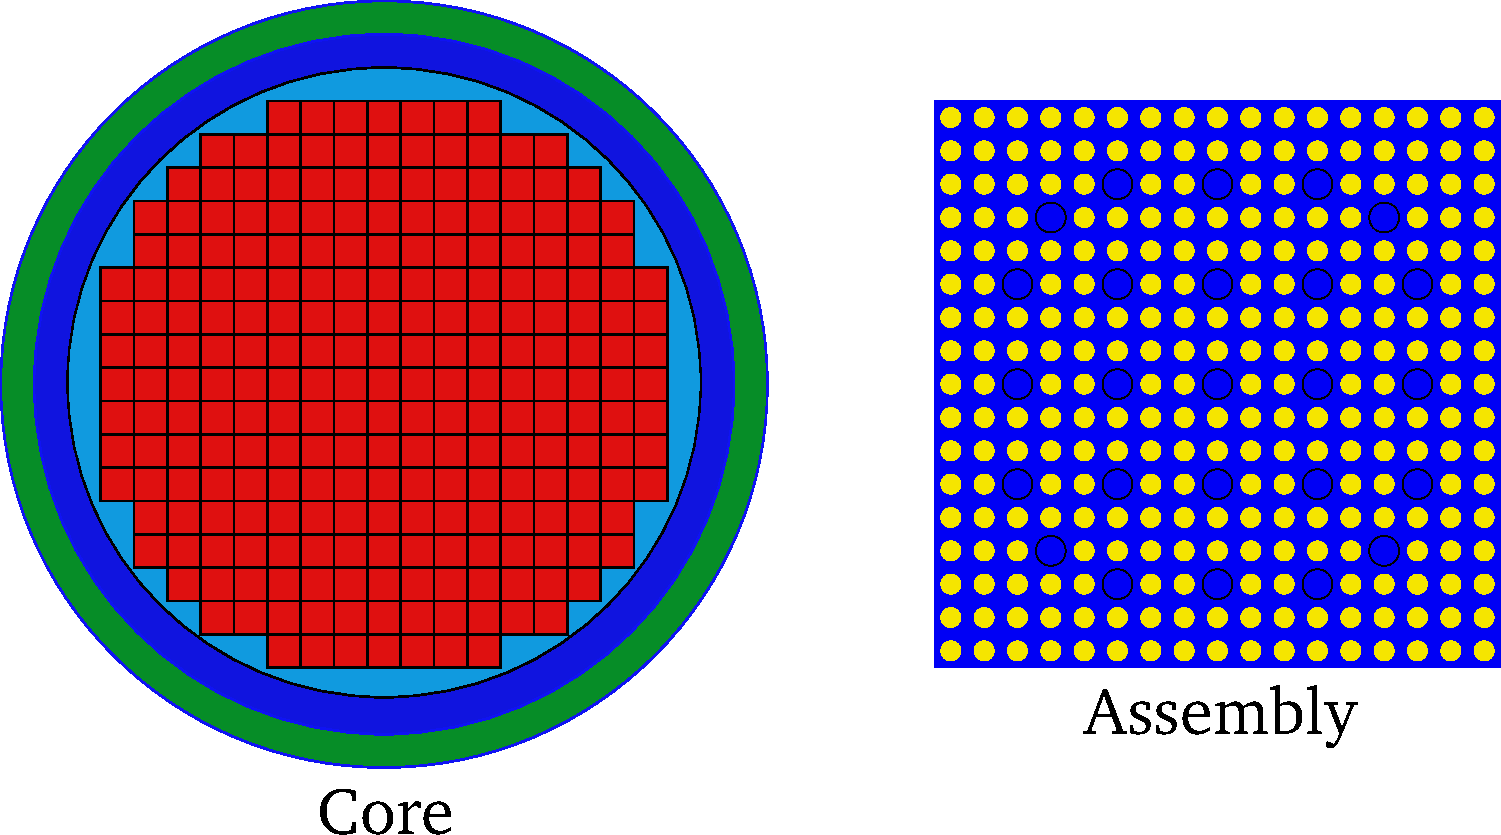
\includegraphics[width=1.7in]{../images/mcperformance.pdf}
    \end{center}
    \footnotesize{
      \begin{itemize}
      \item ALCF Mira supercomputer
      \item 49,152 nodes, 786,432 cores
      \item 4 hw threads/core = 3,145,728 threads
      \end{itemize}
    }
    \column{0.65\textwidth}
    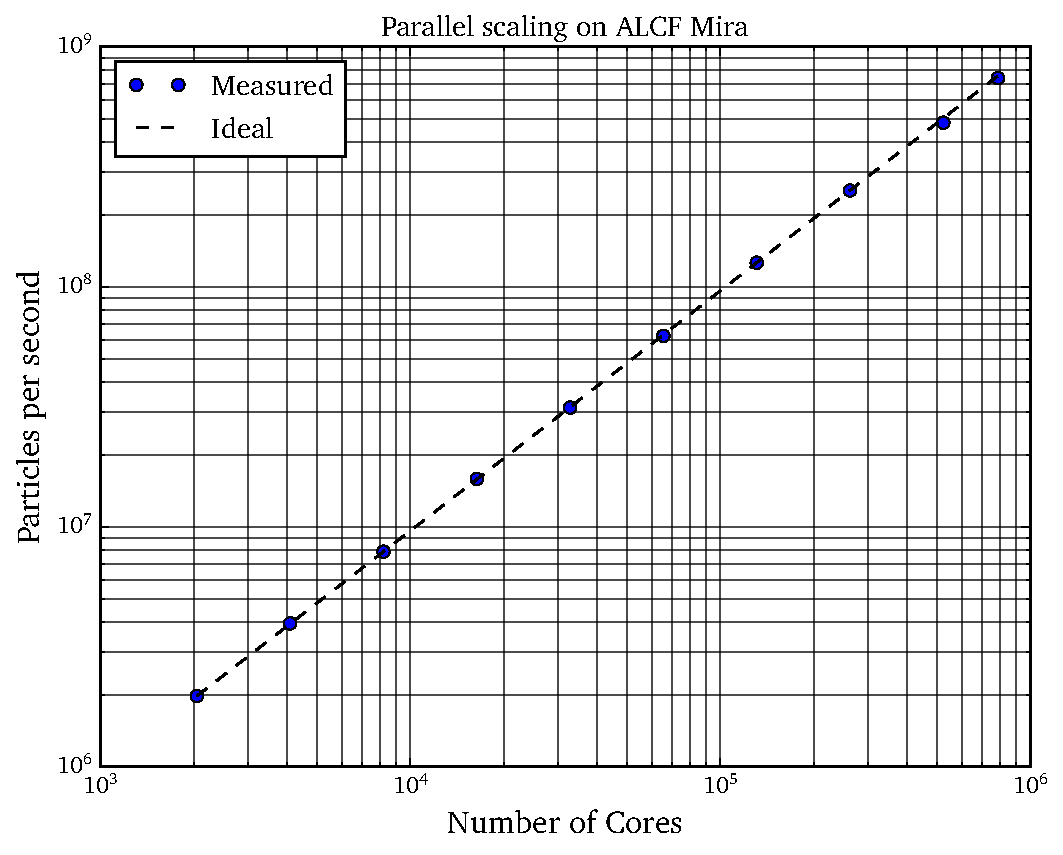
\includegraphics[width=3.0in]{../images/scaling_loglog.pdf}
  \end{columns}
\end{frame}

% \begin{frame}{Validation and Verification}
%   \begin{itemize}
%   \item MCNP Criticality Benchmark Suite
%     \begin{itemize}
%     \item 119 configurations --- different spectra, materials, enrichment
%     \item Models built for all but two
%     \end{itemize}
%   \end{itemize}
%   \centerline{
%     \includegraphics[width=1.35\textwidth]{../images/expanded-suite.pdf}
%   }
% \end{frame}

\begin{frame}{Example: Advanced Test Reactor}
  \begin{center}
    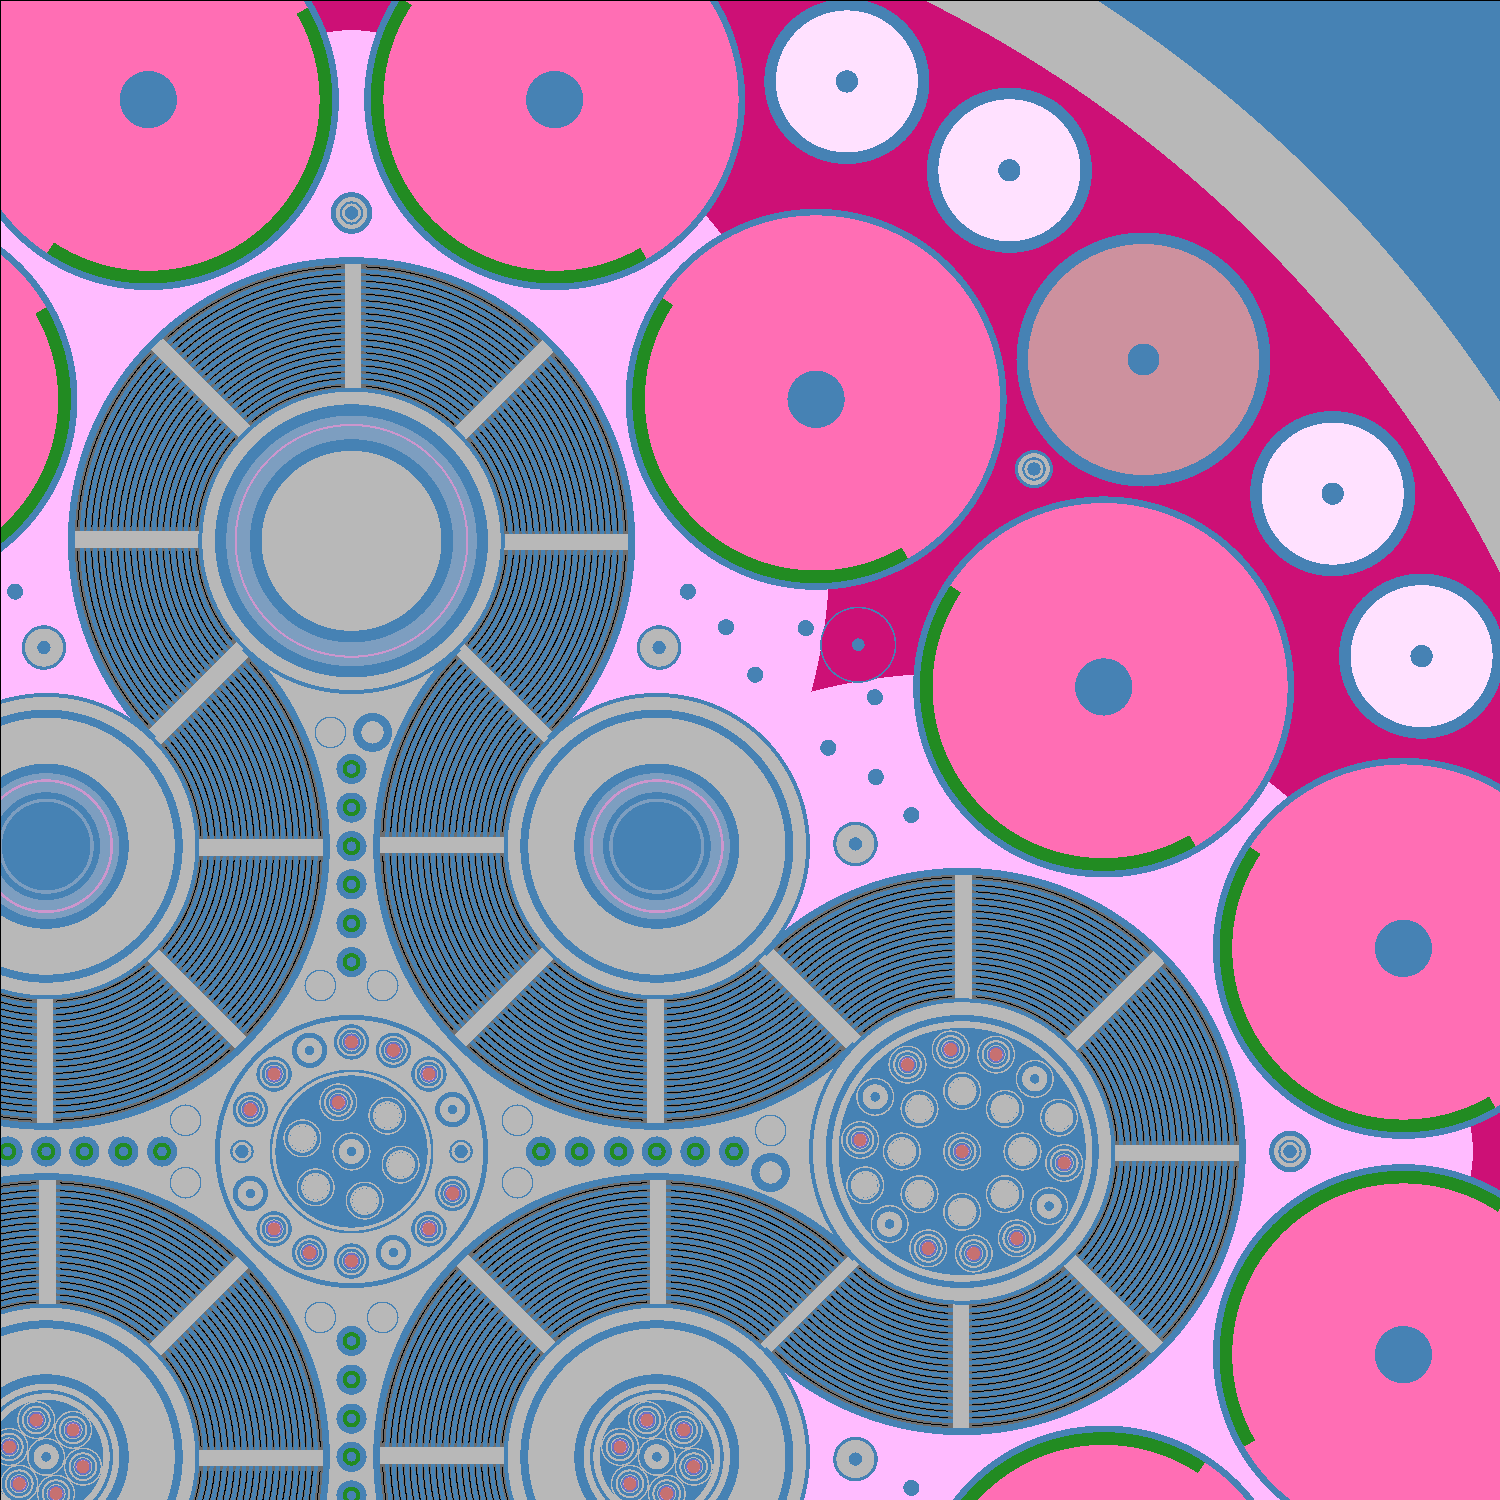
\includegraphics[width=0.7\textwidth]{../images/atr.png}
  \end{center}
\end{frame}

% \begin{frame}{Example: ITER E-Lite}
%   \begin{center}
%     \includegraphics[width=0.7\textwidth]{../images/iter_elite.png}
%   \end{center}
% \end{frame}

\begin{frame}{Software Architecture}
  \begin{itemize}
  \item Mixed \textbf{C++} and \textbf{Python} codebase
  \item \textbf{CMake} build system for portability
  \item Distributed-memory parallelism via \textbf{MPI}
  \item Shared-memory parallelism via \textbf{OpenMP}
  \item Version control through \textbf{git}
  \item Code hosting, bug tracking through \href{https://github.com/openmc-dev/openmc}{\textbf{GitHub}}
  \item Regression/unit tests run on \textbf{GitHub Actions} CI platform
  \end{itemize}
\end{frame}

\begin{frame}{Upcoming developments}
  \begin{itemize}
    \item GPU porting (Exascale Computing Project)
    \item Multiphysics coupling
    \item Fusion shutdown dose rate (SDR) calculations
    \item Unstructured mesh support
    \item Methods to support molten salt reactor design
  \end{itemize}
\end{frame}

\begin{frame}{Resources}
  \begin{itemize}
    \item \textbf{Code:} \url{https://github.com/openmc-dev/openmc}
    \item \textbf{Docs:} \url{https://docs.openmc.org}
    \item \textbf{Nuclear Data:} \url{https://openmc.org}
    \item \textbf{Forum:} \url{https://openmc.discourse.group}
  \end{itemize}
\end{frame}

\end{document}
